
% Default to the notebook output style

    


% Inherit from the specified cell style.




    
\documentclass[11pt]{article}

    
    
    \usepackage[T1]{fontenc}
    % Nicer default font (+ math font) than Computer Modern for most use cases
    \usepackage{mathpazo}

    % Basic figure setup, for now with no caption control since it's done
    % automatically by Pandoc (which extracts ![](path) syntax from Markdown).
    \usepackage{graphicx}
    % We will generate all images so they have a width \maxwidth. This means
    % that they will get their normal width if they fit onto the page, but
    % are scaled down if they would overflow the margins.
    \makeatletter
    \def\maxwidth{\ifdim\Gin@nat@width>\linewidth\linewidth
    \else\Gin@nat@width\fi}
    \makeatother
    \let\Oldincludegraphics\includegraphics
    % Set max figure width to be 80% of text width, for now hardcoded.
    \renewcommand{\includegraphics}[1]{\Oldincludegraphics[width=.8\maxwidth]{#1}}
    % Ensure that by default, figures have no caption (until we provide a
    % proper Figure object with a Caption API and a way to capture that
    % in the conversion process - todo).
    \usepackage{caption}
    \DeclareCaptionLabelFormat{nolabel}{}
    \captionsetup{labelformat=nolabel}

    \usepackage{adjustbox} % Used to constrain images to a maximum size 
    \usepackage{xcolor} % Allow colors to be defined
    \usepackage{enumerate} % Needed for markdown enumerations to work
    \usepackage{geometry} % Used to adjust the document margins
    \usepackage{amsmath} % Equations
    \usepackage{amssymb} % Equations
    \usepackage{textcomp} % defines textquotesingle
    % Hack from http://tex.stackexchange.com/a/47451/13684:
    \AtBeginDocument{%
        \def\PYZsq{\textquotesingle}% Upright quotes in Pygmentized code
    }
    \usepackage{upquote} % Upright quotes for verbatim code
    \usepackage{eurosym} % defines \euro
    \usepackage[mathletters]{ucs} % Extended unicode (utf-8) support
    \usepackage[utf8x]{inputenc} % Allow utf-8 characters in the tex document
    \usepackage{fancyvrb} % verbatim replacement that allows latex
    \usepackage{grffile} % extends the file name processing of package graphics 
                         % to support a larger range 
    % The hyperref package gives us a pdf with properly built
    % internal navigation ('pdf bookmarks' for the table of contents,
    % internal cross-reference links, web links for URLs, etc.)
    \usepackage{hyperref}
    \usepackage{longtable} % longtable support required by pandoc >1.10
    \usepackage{booktabs}  % table support for pandoc > 1.12.2
    \usepackage[inline]{enumitem} % IRkernel/repr support (it uses the enumerate* environment)
    \usepackage[normalem]{ulem} % ulem is needed to support strikethroughs (\sout)
                                % normalem makes italics be italics, not underlines
    

    
    
    % Colors for the hyperref package
    \definecolor{urlcolor}{rgb}{0,.145,.698}
    \definecolor{linkcolor}{rgb}{.71,0.21,0.01}
    \definecolor{citecolor}{rgb}{.12,.54,.11}

    % ANSI colors
    \definecolor{ansi-black}{HTML}{3E424D}
    \definecolor{ansi-black-intense}{HTML}{282C36}
    \definecolor{ansi-red}{HTML}{E75C58}
    \definecolor{ansi-red-intense}{HTML}{B22B31}
    \definecolor{ansi-green}{HTML}{00A250}
    \definecolor{ansi-green-intense}{HTML}{007427}
    \definecolor{ansi-yellow}{HTML}{DDB62B}
    \definecolor{ansi-yellow-intense}{HTML}{B27D12}
    \definecolor{ansi-blue}{HTML}{208FFB}
    \definecolor{ansi-blue-intense}{HTML}{0065CA}
    \definecolor{ansi-magenta}{HTML}{D160C4}
    \definecolor{ansi-magenta-intense}{HTML}{A03196}
    \definecolor{ansi-cyan}{HTML}{60C6C8}
    \definecolor{ansi-cyan-intense}{HTML}{258F8F}
    \definecolor{ansi-white}{HTML}{C5C1B4}
    \definecolor{ansi-white-intense}{HTML}{A1A6B2}

    % commands and environments needed by pandoc snippets
    % extracted from the output of `pandoc -s`
    \providecommand{\tightlist}{%
      \setlength{\itemsep}{0pt}\setlength{\parskip}{0pt}}
    \DefineVerbatimEnvironment{Highlighting}{Verbatim}{commandchars=\\\{\}}
    % Add ',fontsize=\small' for more characters per line
    \newenvironment{Shaded}{}{}
    \newcommand{\KeywordTok}[1]{\textcolor[rgb]{0.00,0.44,0.13}{\textbf{{#1}}}}
    \newcommand{\DataTypeTok}[1]{\textcolor[rgb]{0.56,0.13,0.00}{{#1}}}
    \newcommand{\DecValTok}[1]{\textcolor[rgb]{0.25,0.63,0.44}{{#1}}}
    \newcommand{\BaseNTok}[1]{\textcolor[rgb]{0.25,0.63,0.44}{{#1}}}
    \newcommand{\FloatTok}[1]{\textcolor[rgb]{0.25,0.63,0.44}{{#1}}}
    \newcommand{\CharTok}[1]{\textcolor[rgb]{0.25,0.44,0.63}{{#1}}}
    \newcommand{\StringTok}[1]{\textcolor[rgb]{0.25,0.44,0.63}{{#1}}}
    \newcommand{\CommentTok}[1]{\textcolor[rgb]{0.38,0.63,0.69}{\textit{{#1}}}}
    \newcommand{\OtherTok}[1]{\textcolor[rgb]{0.00,0.44,0.13}{{#1}}}
    \newcommand{\AlertTok}[1]{\textcolor[rgb]{1.00,0.00,0.00}{\textbf{{#1}}}}
    \newcommand{\FunctionTok}[1]{\textcolor[rgb]{0.02,0.16,0.49}{{#1}}}
    \newcommand{\RegionMarkerTok}[1]{{#1}}
    \newcommand{\ErrorTok}[1]{\textcolor[rgb]{1.00,0.00,0.00}{\textbf{{#1}}}}
    \newcommand{\NormalTok}[1]{{#1}}
    
    % Additional commands for more recent versions of Pandoc
    \newcommand{\ConstantTok}[1]{\textcolor[rgb]{0.53,0.00,0.00}{{#1}}}
    \newcommand{\SpecialCharTok}[1]{\textcolor[rgb]{0.25,0.44,0.63}{{#1}}}
    \newcommand{\VerbatimStringTok}[1]{\textcolor[rgb]{0.25,0.44,0.63}{{#1}}}
    \newcommand{\SpecialStringTok}[1]{\textcolor[rgb]{0.73,0.40,0.53}{{#1}}}
    \newcommand{\ImportTok}[1]{{#1}}
    \newcommand{\DocumentationTok}[1]{\textcolor[rgb]{0.73,0.13,0.13}{\textit{{#1}}}}
    \newcommand{\AnnotationTok}[1]{\textcolor[rgb]{0.38,0.63,0.69}{\textbf{\textit{{#1}}}}}
    \newcommand{\CommentVarTok}[1]{\textcolor[rgb]{0.38,0.63,0.69}{\textbf{\textit{{#1}}}}}
    \newcommand{\VariableTok}[1]{\textcolor[rgb]{0.10,0.09,0.49}{{#1}}}
    \newcommand{\ControlFlowTok}[1]{\textcolor[rgb]{0.00,0.44,0.13}{\textbf{{#1}}}}
    \newcommand{\OperatorTok}[1]{\textcolor[rgb]{0.40,0.40,0.40}{{#1}}}
    \newcommand{\BuiltInTok}[1]{{#1}}
    \newcommand{\ExtensionTok}[1]{{#1}}
    \newcommand{\PreprocessorTok}[1]{\textcolor[rgb]{0.74,0.48,0.00}{{#1}}}
    \newcommand{\AttributeTok}[1]{\textcolor[rgb]{0.49,0.56,0.16}{{#1}}}
    \newcommand{\InformationTok}[1]{\textcolor[rgb]{0.38,0.63,0.69}{\textbf{\textit{{#1}}}}}
    \newcommand{\WarningTok}[1]{\textcolor[rgb]{0.38,0.63,0.69}{\textbf{\textit{{#1}}}}}
    
    
    % Define a nice break command that doesn't care if a line doesn't already
    % exist.
    \def\br{\hspace*{\fill} \\* }
    % Math Jax compatability definitions
    \def\gt{>}
    \def\lt{<}
    % Document parameters
    \title{lecture\_12}
    
    
    

    % Pygments definitions
    
\makeatletter
\def\PY@reset{\let\PY@it=\relax \let\PY@bf=\relax%
    \let\PY@ul=\relax \let\PY@tc=\relax%
    \let\PY@bc=\relax \let\PY@ff=\relax}
\def\PY@tok#1{\csname PY@tok@#1\endcsname}
\def\PY@toks#1+{\ifx\relax#1\empty\else%
    \PY@tok{#1}\expandafter\PY@toks\fi}
\def\PY@do#1{\PY@bc{\PY@tc{\PY@ul{%
    \PY@it{\PY@bf{\PY@ff{#1}}}}}}}
\def\PY#1#2{\PY@reset\PY@toks#1+\relax+\PY@do{#2}}

\expandafter\def\csname PY@tok@gd\endcsname{\def\PY@tc##1{\textcolor[rgb]{0.63,0.00,0.00}{##1}}}
\expandafter\def\csname PY@tok@gu\endcsname{\let\PY@bf=\textbf\def\PY@tc##1{\textcolor[rgb]{0.50,0.00,0.50}{##1}}}
\expandafter\def\csname PY@tok@gt\endcsname{\def\PY@tc##1{\textcolor[rgb]{0.00,0.27,0.87}{##1}}}
\expandafter\def\csname PY@tok@gs\endcsname{\let\PY@bf=\textbf}
\expandafter\def\csname PY@tok@gr\endcsname{\def\PY@tc##1{\textcolor[rgb]{1.00,0.00,0.00}{##1}}}
\expandafter\def\csname PY@tok@cm\endcsname{\let\PY@it=\textit\def\PY@tc##1{\textcolor[rgb]{0.25,0.50,0.50}{##1}}}
\expandafter\def\csname PY@tok@vg\endcsname{\def\PY@tc##1{\textcolor[rgb]{0.10,0.09,0.49}{##1}}}
\expandafter\def\csname PY@tok@vi\endcsname{\def\PY@tc##1{\textcolor[rgb]{0.10,0.09,0.49}{##1}}}
\expandafter\def\csname PY@tok@mh\endcsname{\def\PY@tc##1{\textcolor[rgb]{0.40,0.40,0.40}{##1}}}
\expandafter\def\csname PY@tok@cs\endcsname{\let\PY@it=\textit\def\PY@tc##1{\textcolor[rgb]{0.25,0.50,0.50}{##1}}}
\expandafter\def\csname PY@tok@ge\endcsname{\let\PY@it=\textit}
\expandafter\def\csname PY@tok@vc\endcsname{\def\PY@tc##1{\textcolor[rgb]{0.10,0.09,0.49}{##1}}}
\expandafter\def\csname PY@tok@il\endcsname{\def\PY@tc##1{\textcolor[rgb]{0.40,0.40,0.40}{##1}}}
\expandafter\def\csname PY@tok@go\endcsname{\def\PY@tc##1{\textcolor[rgb]{0.53,0.53,0.53}{##1}}}
\expandafter\def\csname PY@tok@cp\endcsname{\def\PY@tc##1{\textcolor[rgb]{0.74,0.48,0.00}{##1}}}
\expandafter\def\csname PY@tok@gi\endcsname{\def\PY@tc##1{\textcolor[rgb]{0.00,0.63,0.00}{##1}}}
\expandafter\def\csname PY@tok@gh\endcsname{\let\PY@bf=\textbf\def\PY@tc##1{\textcolor[rgb]{0.00,0.00,0.50}{##1}}}
\expandafter\def\csname PY@tok@ni\endcsname{\let\PY@bf=\textbf\def\PY@tc##1{\textcolor[rgb]{0.60,0.60,0.60}{##1}}}
\expandafter\def\csname PY@tok@nl\endcsname{\def\PY@tc##1{\textcolor[rgb]{0.63,0.63,0.00}{##1}}}
\expandafter\def\csname PY@tok@nn\endcsname{\let\PY@bf=\textbf\def\PY@tc##1{\textcolor[rgb]{0.00,0.00,1.00}{##1}}}
\expandafter\def\csname PY@tok@no\endcsname{\def\PY@tc##1{\textcolor[rgb]{0.53,0.00,0.00}{##1}}}
\expandafter\def\csname PY@tok@na\endcsname{\def\PY@tc##1{\textcolor[rgb]{0.49,0.56,0.16}{##1}}}
\expandafter\def\csname PY@tok@nb\endcsname{\def\PY@tc##1{\textcolor[rgb]{0.00,0.50,0.00}{##1}}}
\expandafter\def\csname PY@tok@nc\endcsname{\let\PY@bf=\textbf\def\PY@tc##1{\textcolor[rgb]{0.00,0.00,1.00}{##1}}}
\expandafter\def\csname PY@tok@nd\endcsname{\def\PY@tc##1{\textcolor[rgb]{0.67,0.13,1.00}{##1}}}
\expandafter\def\csname PY@tok@ne\endcsname{\let\PY@bf=\textbf\def\PY@tc##1{\textcolor[rgb]{0.82,0.25,0.23}{##1}}}
\expandafter\def\csname PY@tok@nf\endcsname{\def\PY@tc##1{\textcolor[rgb]{0.00,0.00,1.00}{##1}}}
\expandafter\def\csname PY@tok@si\endcsname{\let\PY@bf=\textbf\def\PY@tc##1{\textcolor[rgb]{0.73,0.40,0.53}{##1}}}
\expandafter\def\csname PY@tok@s2\endcsname{\def\PY@tc##1{\textcolor[rgb]{0.73,0.13,0.13}{##1}}}
\expandafter\def\csname PY@tok@nt\endcsname{\let\PY@bf=\textbf\def\PY@tc##1{\textcolor[rgb]{0.00,0.50,0.00}{##1}}}
\expandafter\def\csname PY@tok@nv\endcsname{\def\PY@tc##1{\textcolor[rgb]{0.10,0.09,0.49}{##1}}}
\expandafter\def\csname PY@tok@s1\endcsname{\def\PY@tc##1{\textcolor[rgb]{0.73,0.13,0.13}{##1}}}
\expandafter\def\csname PY@tok@ch\endcsname{\let\PY@it=\textit\def\PY@tc##1{\textcolor[rgb]{0.25,0.50,0.50}{##1}}}
\expandafter\def\csname PY@tok@m\endcsname{\def\PY@tc##1{\textcolor[rgb]{0.40,0.40,0.40}{##1}}}
\expandafter\def\csname PY@tok@gp\endcsname{\let\PY@bf=\textbf\def\PY@tc##1{\textcolor[rgb]{0.00,0.00,0.50}{##1}}}
\expandafter\def\csname PY@tok@sh\endcsname{\def\PY@tc##1{\textcolor[rgb]{0.73,0.13,0.13}{##1}}}
\expandafter\def\csname PY@tok@ow\endcsname{\let\PY@bf=\textbf\def\PY@tc##1{\textcolor[rgb]{0.67,0.13,1.00}{##1}}}
\expandafter\def\csname PY@tok@sx\endcsname{\def\PY@tc##1{\textcolor[rgb]{0.00,0.50,0.00}{##1}}}
\expandafter\def\csname PY@tok@bp\endcsname{\def\PY@tc##1{\textcolor[rgb]{0.00,0.50,0.00}{##1}}}
\expandafter\def\csname PY@tok@c1\endcsname{\let\PY@it=\textit\def\PY@tc##1{\textcolor[rgb]{0.25,0.50,0.50}{##1}}}
\expandafter\def\csname PY@tok@o\endcsname{\def\PY@tc##1{\textcolor[rgb]{0.40,0.40,0.40}{##1}}}
\expandafter\def\csname PY@tok@kc\endcsname{\let\PY@bf=\textbf\def\PY@tc##1{\textcolor[rgb]{0.00,0.50,0.00}{##1}}}
\expandafter\def\csname PY@tok@c\endcsname{\let\PY@it=\textit\def\PY@tc##1{\textcolor[rgb]{0.25,0.50,0.50}{##1}}}
\expandafter\def\csname PY@tok@mf\endcsname{\def\PY@tc##1{\textcolor[rgb]{0.40,0.40,0.40}{##1}}}
\expandafter\def\csname PY@tok@err\endcsname{\def\PY@bc##1{\setlength{\fboxsep}{0pt}\fcolorbox[rgb]{1.00,0.00,0.00}{1,1,1}{\strut ##1}}}
\expandafter\def\csname PY@tok@mb\endcsname{\def\PY@tc##1{\textcolor[rgb]{0.40,0.40,0.40}{##1}}}
\expandafter\def\csname PY@tok@ss\endcsname{\def\PY@tc##1{\textcolor[rgb]{0.10,0.09,0.49}{##1}}}
\expandafter\def\csname PY@tok@sr\endcsname{\def\PY@tc##1{\textcolor[rgb]{0.73,0.40,0.53}{##1}}}
\expandafter\def\csname PY@tok@mo\endcsname{\def\PY@tc##1{\textcolor[rgb]{0.40,0.40,0.40}{##1}}}
\expandafter\def\csname PY@tok@kd\endcsname{\let\PY@bf=\textbf\def\PY@tc##1{\textcolor[rgb]{0.00,0.50,0.00}{##1}}}
\expandafter\def\csname PY@tok@mi\endcsname{\def\PY@tc##1{\textcolor[rgb]{0.40,0.40,0.40}{##1}}}
\expandafter\def\csname PY@tok@kn\endcsname{\let\PY@bf=\textbf\def\PY@tc##1{\textcolor[rgb]{0.00,0.50,0.00}{##1}}}
\expandafter\def\csname PY@tok@cpf\endcsname{\let\PY@it=\textit\def\PY@tc##1{\textcolor[rgb]{0.25,0.50,0.50}{##1}}}
\expandafter\def\csname PY@tok@kr\endcsname{\let\PY@bf=\textbf\def\PY@tc##1{\textcolor[rgb]{0.00,0.50,0.00}{##1}}}
\expandafter\def\csname PY@tok@s\endcsname{\def\PY@tc##1{\textcolor[rgb]{0.73,0.13,0.13}{##1}}}
\expandafter\def\csname PY@tok@kp\endcsname{\def\PY@tc##1{\textcolor[rgb]{0.00,0.50,0.00}{##1}}}
\expandafter\def\csname PY@tok@w\endcsname{\def\PY@tc##1{\textcolor[rgb]{0.73,0.73,0.73}{##1}}}
\expandafter\def\csname PY@tok@kt\endcsname{\def\PY@tc##1{\textcolor[rgb]{0.69,0.00,0.25}{##1}}}
\expandafter\def\csname PY@tok@sc\endcsname{\def\PY@tc##1{\textcolor[rgb]{0.73,0.13,0.13}{##1}}}
\expandafter\def\csname PY@tok@sb\endcsname{\def\PY@tc##1{\textcolor[rgb]{0.73,0.13,0.13}{##1}}}
\expandafter\def\csname PY@tok@k\endcsname{\let\PY@bf=\textbf\def\PY@tc##1{\textcolor[rgb]{0.00,0.50,0.00}{##1}}}
\expandafter\def\csname PY@tok@se\endcsname{\let\PY@bf=\textbf\def\PY@tc##1{\textcolor[rgb]{0.73,0.40,0.13}{##1}}}
\expandafter\def\csname PY@tok@sd\endcsname{\let\PY@it=\textit\def\PY@tc##1{\textcolor[rgb]{0.73,0.13,0.13}{##1}}}

\def\PYZbs{\char`\\}
\def\PYZus{\char`\_}
\def\PYZob{\char`\{}
\def\PYZcb{\char`\}}
\def\PYZca{\char`\^}
\def\PYZam{\char`\&}
\def\PYZlt{\char`\<}
\def\PYZgt{\char`\>}
\def\PYZsh{\char`\#}
\def\PYZpc{\char`\%}
\def\PYZdl{\char`\$}
\def\PYZhy{\char`\-}
\def\PYZsq{\char`\'}
\def\PYZdq{\char`\"}
\def\PYZti{\char`\~}
% for compatibility with earlier versions
\def\PYZat{@}
\def\PYZlb{[}
\def\PYZrb{]}
\makeatother


    % Exact colors from NB
    \definecolor{incolor}{rgb}{0.0, 0.0, 0.5}
    \definecolor{outcolor}{rgb}{0.545, 0.0, 0.0}



    
    % Prevent overflowing lines due to hard-to-break entities
    \sloppy 
    % Setup hyperref package
    \hypersetup{
      breaklinks=true,  % so long urls are correctly broken across lines
      colorlinks=true,
      urlcolor=urlcolor,
      linkcolor=linkcolor,
      citecolor=citecolor,
      }
    % Slightly bigger margins than the latex defaults
    
    \geometry{verbose,tmargin=1in,bmargin=1in,lmargin=1in,rmargin=1in}
    
    

    \begin{document}
    
    
    \maketitle
    
    

    
    \begin{Verbatim}[commandchars=\\\{\}]
{\color{incolor}In [{\color{incolor}27}]:} \PY{c}{\PYZpc{}plot \PYZhy{}\PYZhy{}format svg}
\end{Verbatim}

    \begin{Verbatim}[commandchars=\\\{\}]
{\color{incolor}In [{\color{incolor}28}]:} \PY{n}{setdefaults}
\end{Verbatim}

    \begin{Verbatim}[commandchars=\\\{\}]
{\color{incolor}In [{\color{incolor}29}]:} \PY{n}{A}\PY{p}{=}\PY{n+nb}{rand}\PY{p}{(}\PY{l+m+mi}{4}\PY{p}{,}\PY{l+m+mi}{4}\PY{p}{)}
         
         \PY{p}{[}\PY{n}{L}\PY{p}{,}\PY{n}{U}\PY{p}{,}\PY{n}{P}\PY{p}{]}\PY{p}{=}\PY{n+nb}{lu}\PY{p}{(}\PY{n}{A}\PY{p}{)}
         
         \PY{n+nb}{det}\PY{p}{(}\PY{n}{L}\PY{p}{)}
\end{Verbatim}

    \begin{Verbatim}[commandchars=\\\{\}]
A =

   0.447394   0.357071   0.720915   0.499926
   0.648313   0.323276   0.521677   0.288345
   0.084982   0.581513   0.466420   0.142342
   0.576580   0.658089   0.916987   0.923165

L =

   1.00000   0.00000   0.00000   0.00000
   0.13108   1.00000   0.00000   0.00000
   0.69009   0.24851   1.00000   0.00000
   0.88935   0.68736   0.68488   1.00000

U =

   0.64831   0.32328   0.52168   0.28834
   0.00000   0.53914   0.39804   0.10455
   0.00000   0.00000   0.26199   0.27496
   0.00000   0.00000   0.00000   0.40655

P =

Permutation Matrix

   0   1   0   0
   0   0   1   0
   1   0   0   0
   0   0   0   1

ans =  1

    \end{Verbatim}

    \begin{Verbatim}[commandchars=\\\{\}]
{\color{incolor}In [{\color{incolor}44}]:} \PY{n}{A}\PY{p}{=}\PY{n+nb}{rand}\PY{p}{(}\PY{l+m+mi}{4}\PY{p}{,}\PY{l+m+mi}{100}\PY{p}{)}\PY{o}{\PYZsq{}}\PY{p}{;}
         \PY{n}{A}\PY{p}{=}\PY{n}{A}\PY{o}{\PYZsq{}}\PY{o}{*}\PY{n}{A}\PY{p}{;}
         \PY{n+nb}{size}\PY{p}{(}\PY{n}{A}\PY{p}{)}
         \PY{n+nb}{min}\PY{p}{(}\PY{n+nb}{min}\PY{p}{(}\PY{n}{A}\PY{p}{)}\PY{p}{)}
         \PY{n+nb}{max}\PY{p}{(}\PY{n+nb}{max}\PY{p}{(}\PY{n}{A}\PY{p}{)}\PY{p}{)}
         \PY{n+nb}{cond}\PY{p}{(}\PY{n}{A}\PY{p}{)}
         \PY{n}{C}\PY{p}{=}\PY{n+nb}{chol}\PY{p}{(}\PY{n}{A}\PY{p}{)}
\end{Verbatim}

    \begin{Verbatim}[commandchars=\\\{\}]
ans =

   4   4

ans =  23.586
ans =  35.826
ans =  14.869
C =

   5.98549   4.28555   4.35707   4.31359
   0.00000   3.63950   1.35005   1.45342
   0.00000   0.00000   3.62851   1.50580
   0.00000   0.00000   0.00000   3.21911


    \end{Verbatim}

    \subsection{My question from last
class}\label{my-question-from-last-class}

\begin{figure}[htbp]
\centering
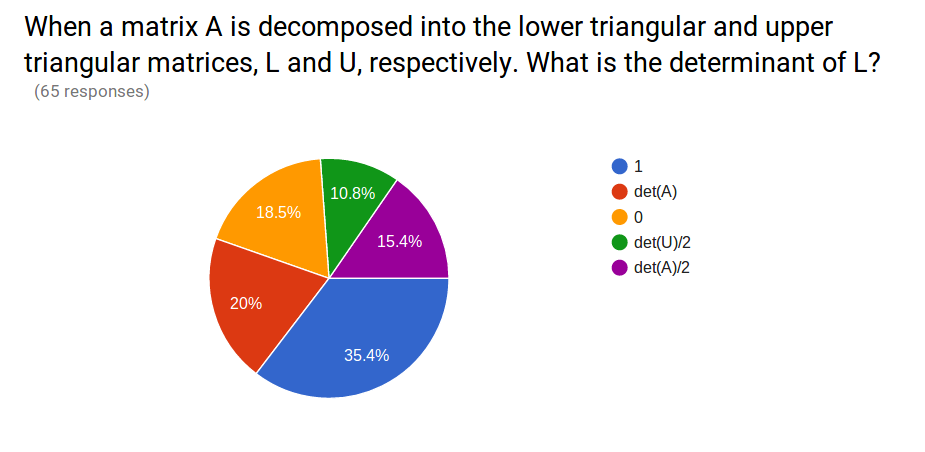
\includegraphics{det_L.png}
\caption{q1}
\end{figure}

\begin{figure}[htbp]
\centering
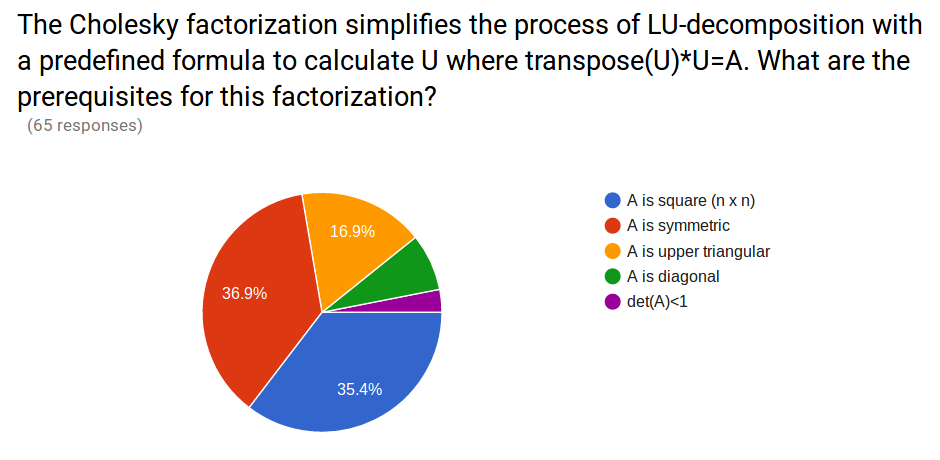
\includegraphics{chol_pre.png}
\caption{q2}
\end{figure}

\subsection{Your questions from last
class}\label{your-questions-from-last-class}

\begin{enumerate}
\def\labelenumi{\arabic{enumi}.}
\item
  Will the exam be more theoretical or problem based?
\item
  Writing code is difficult
\item
  What format can we expect for the midterm?
\item
  Could we go over some example questions for the exam?
\item
  Will the use of GitHub be tested on the Midterm exam? Or is it more
  focused on linear algebra techniques/what was covered in the lectures?
\item
  This is not my strong suit, getting a bit overwhelmed with matrix
  multiplication.
\item
  I forgot how much I learned in linear algebra.
\item
  What's the most exciting project you've ever worked on with
  Matlab/Octave?
\end{enumerate}

    \section{Matrix Inverse and
Condition}\label{matrix-inverse-and-condition}

Considering the same solution set:

\(y=Ax\)

If we know that \(A^{-1}A=I\), then

\(A^{-1}y=A^{-1}Ax=x\)

so

\(x=A^{-1}y\)

Where, \(A^{-1}\) is the inverse of matrix \(A\).

\(2x_{1}+x_{2}=1\)

\(x_{1}+3x_{2}=1\)

\(Ax=y\)

\(\left[ \begin{array}{cc} 2 & 1 \\ 1 & 3 \end{array} \right] \left[\begin{array}{c} x_{1} \\ x_{2} \end{array}\right]= \left[\begin{array}{c} 1 \\ 1\end{array}\right]\)

\(A^{-1}=\frac{1}{2*3-1*1}\left[ \begin{array}{cc} 3 & -1 \\ -1 & 2 \end{array} \right]= \left[ \begin{array}{cc} 3/5 & -1/5 \\ -1/5 & 2/5 \end{array} \right]\)

    \begin{Verbatim}[commandchars=\\\{\}]
{\color{incolor}In [{\color{incolor}45}]:} \PY{n}{A}\PY{p}{=}\PY{p}{[}\PY{l+m+mi}{2}\PY{p}{,}\PY{l+m+mi}{1}\PY{p}{;}\PY{l+m+mi}{1}\PY{p}{,}\PY{l+m+mi}{3}\PY{p}{]}
         \PY{n}{invA}\PY{p}{=}\PY{l+m+mi}{1}\PY{o}{/}\PY{l+m+mi}{5}\PY{o}{*}\PY{p}{[}\PY{l+m+mi}{3}\PY{p}{,}\PY{o}{\PYZhy{}}\PY{l+m+mi}{1}\PY{p}{;}\PY{o}{\PYZhy{}}\PY{l+m+mi}{1}\PY{p}{,}\PY{l+m+mi}{2}\PY{p}{]}
         
         \PY{n}{A}\PY{o}{*}\PY{n}{invA}
         \PY{n}{invA}\PY{o}{*}\PY{n}{A}
\end{Verbatim}

    \begin{Verbatim}[commandchars=\\\{\}]
A =

   2   1
   1   3

invA =

   0.60000  -0.20000
  -0.20000   0.40000

ans =

   1.00000   0.00000
   0.00000   1.00000

ans =

   1.00000   0.00000
   0.00000   1.00000


    \end{Verbatim}

    How did we know the inverse of A?

for 2$\times$2 matrices, it is always:

$A=\left[ \begin{array}{cc} A_{11} & A_{12} \\ A_{21} & A_{22} \end{array} \right]$

$A^{-1}=\frac{1}{det(A)}\left[ \begin{array}{cc} A_{22} & -A_{12} \\ -A_{21} & A_{11} \end{array} \right]$

    $AA^{-1}=\frac{1}{A_{11}A_{22}-A_{21}A_{12}}\left[ \begin{array}{cc} A_{11}A_{22}-A_{21}A_{12} & -A_{11}A_{12}+A_{12}A_{11} \\ A_{21}A_{22}-A_{22}A_{21} & -A_{21}A_{12}+A_{22}A_{11} \end{array} \right] =\left[ \begin{array}{cc} 1 & 0 \\ 0 & 1 \end{array} \right]$

    What about bigger matrices?

We can use the LU-decomposition

\(A=LU\)

\(A^{-1}=(LU)^{-1}=U^{-1}L^{-1}\)

if we divide \(A^{-1}\) into n-column vectors, \(a_{n}\), then

\(Aa_{1}=\left[\begin{array}{c} 1 \\ 0 \\ \vdots \\ 0 \end{array} \right]\)
\(Aa_{2}=\left[\begin{array}{c} 0 \\ 1 \\ \vdots \\ 0 \end{array} \right]\)
\(Aa_{n}=\left[\begin{array}{c} 0 \\ 0 \\ \vdots \\ 1 \end{array} \right]\)

Which we can solve for each \(a_{n}\) with LU-decomposition, knowing the
lower and upper triangular decompositions, then

\(A^{-1}=\left[ \begin{array}{cccc} | & | & & | \\ a_{1} & a_{2} & \cdots & a_{n} \\ | & | & & | \end{array} \right]\)

\(Ld_{1}=\left[\begin{array}{c} 1 \\ 0 \\ \vdots \\ 0 \end{array} \right]\)
\(;~Ua_{1}=d_{1}\)

\(Ld_{2}=\left[\begin{array}{c} 0 \\ 1 \\ \vdots \\ 0 \end{array} \right]\)
\(;~Ua_{2}=d_{2}\)

\(Ld_{n}=\left[\begin{array}{c} 0 \\ 1 \\ \vdots \\ n \end{array} \right]\)
\(;~Ua_{n}=d_{n}\)

Consider the following matrix:

\(A=\left[ \begin{array}{ccc} 2 & -1 & 0\\ -1 & 2 & -1\\ 0 & -1 & 1 \end{array} \right]\)

    \paragraph{\texorpdfstring{Note on solving for \(A^{-1}\) column
1}{Note on solving for A\^{}\{-1\} column 1}}\label{note-on-solving-for-a-1-column-1}

\(Aa_1=I(:,1)\)

\(LUa_1=I(:,1)\)

\((LUa_1-I(:,1))=0\)

\(L(Ua_1-d_1)=0\)

\(I(:,1)=Ld_1\)

    \begin{Verbatim}[commandchars=\\\{\}]
{\color{incolor}In [{\color{incolor}56}]:} \PY{n}{A}\PY{p}{=}\PY{p}{[}\PY{l+m+mi}{2}\PY{p}{,}\PY{o}{\PYZhy{}}\PY{l+m+mi}{1}\PY{p}{,}\PY{l+m+mi}{0}\PY{p}{;}\PY{o}{\PYZhy{}}\PY{l+m+mi}{1}\PY{p}{,}\PY{l+m+mi}{2}\PY{p}{,}\PY{o}{\PYZhy{}}\PY{l+m+mi}{1}\PY{p}{;}\PY{l+m+mi}{0}\PY{p}{,}\PY{o}{\PYZhy{}}\PY{l+m+mi}{1}\PY{p}{,}\PY{l+m+mi}{1}\PY{p}{]}
         \PY{n}{U}\PY{p}{=}\PY{n}{A}\PY{p}{;}
         \PY{n}{L}\PY{p}{=}\PY{n+nb}{eye}\PY{p}{(}\PY{l+m+mi}{3}\PY{p}{,}\PY{l+m+mi}{3}\PY{p}{)}\PY{p}{;}
         \PY{n}{U}\PY{p}{(}\PY{l+m+mi}{2}\PY{p}{,}\PY{p}{:}\PY{p}{)}\PY{p}{=}\PY{n}{U}\PY{p}{(}\PY{l+m+mi}{2}\PY{p}{,}\PY{p}{:}\PY{p}{)}\PY{o}{\PYZhy{}}\PY{n}{U}\PY{p}{(}\PY{l+m+mi}{2}\PY{p}{,}\PY{l+m+mi}{1}\PY{p}{)}\PY{o}{/}\PY{n}{U}\PY{p}{(}\PY{l+m+mi}{1}\PY{p}{,}\PY{l+m+mi}{1}\PY{p}{)}\PY{o}{*}\PY{n}{U}\PY{p}{(}\PY{l+m+mi}{1}\PY{p}{,}\PY{p}{:}\PY{p}{)}
         \PY{n}{L}\PY{p}{(}\PY{l+m+mi}{2}\PY{p}{,}\PY{l+m+mi}{1}\PY{p}{)}\PY{p}{=}\PY{n}{A}\PY{p}{(}\PY{l+m+mi}{2}\PY{p}{,}\PY{l+m+mi}{1}\PY{p}{)}\PY{o}{/}\PY{n}{A}\PY{p}{(}\PY{l+m+mi}{1}\PY{p}{,}\PY{l+m+mi}{1}\PY{p}{)}
\end{Verbatim}

    \begin{Verbatim}[commandchars=\\\{\}]
A =

   2  -1   0
  -1   2  -1
   0  -1   1

U =

   2.00000  -1.00000   0.00000
   0.00000   1.50000  -1.00000
   0.00000  -1.00000   1.00000

L =

   1.00000   0.00000   0.00000
  -0.50000   1.00000   0.00000
   0.00000   0.00000   1.00000


    \end{Verbatim}

    \begin{Verbatim}[commandchars=\\\{\}]
{\color{incolor}In [{\color{incolor}57}]:} \PY{n}{L}\PY{p}{(}\PY{l+m+mi}{3}\PY{p}{,}\PY{l+m+mi}{2}\PY{p}{)}\PY{p}{=}\PY{n}{U}\PY{p}{(}\PY{l+m+mi}{3}\PY{p}{,}\PY{l+m+mi}{2}\PY{p}{)}\PY{o}{/}\PY{n}{U}\PY{p}{(}\PY{l+m+mi}{2}\PY{p}{,}\PY{l+m+mi}{2}\PY{p}{)}
         \PY{n}{U}\PY{p}{(}\PY{l+m+mi}{3}\PY{p}{,}\PY{p}{:}\PY{p}{)}\PY{p}{=}\PY{n}{U}\PY{p}{(}\PY{l+m+mi}{3}\PY{p}{,}\PY{p}{:}\PY{p}{)}\PY{o}{\PYZhy{}}\PY{n}{U}\PY{p}{(}\PY{l+m+mi}{3}\PY{p}{,}\PY{l+m+mi}{2}\PY{p}{)}\PY{o}{/}\PY{n}{U}\PY{p}{(}\PY{l+m+mi}{2}\PY{p}{,}\PY{l+m+mi}{2}\PY{p}{)}\PY{o}{*}\PY{n}{U}\PY{p}{(}\PY{l+m+mi}{2}\PY{p}{,}\PY{p}{:}\PY{p}{)}
\end{Verbatim}

    \begin{Verbatim}[commandchars=\\\{\}]
L =

   1.00000   0.00000   0.00000
  -0.50000   1.00000   0.00000
   0.00000  -0.66667   1.00000

U =

   2.00000  -1.00000   0.00000
   0.00000   1.50000  -1.00000
   0.00000   0.00000   0.33333


    \end{Verbatim}

    Now solve for \(d_1\) then \(a_1\), \(d_2\) then \(a_2\), and \(d_3\)
then \(a_{3}\)

\(Ld_{1}=\left[\begin{array}{c} 1 \\ 0 \\ \vdots \\ 0 \end{array} \right]= \left[\begin{array}{ccc} 1 & 0 & 0 \\ -1/2 & 1 & 0 \\ 0 & -2/3 & 1 \end{array} \right]\left[\begin{array}{c} d1(1) \\ d1(2) \\ d1(3)\end{array} \right]=\left[\begin{array}{c} 1 \\ 0 \\ 0 \end{array} \right] ;~Ua_{1}=d_{1}\)

    \begin{Verbatim}[commandchars=\\\{\}]
{\color{incolor}In [{\color{incolor}58}]:} \PY{n}{d1}\PY{p}{=}\PY{n+nb}{zeros}\PY{p}{(}\PY{l+m+mi}{3}\PY{p}{,}\PY{l+m+mi}{1}\PY{p}{)}\PY{p}{;}
         \PY{n}{d1}\PY{p}{(}\PY{l+m+mi}{1}\PY{p}{)}\PY{p}{=}\PY{l+m+mi}{1}\PY{p}{;}
         \PY{n}{d1}\PY{p}{(}\PY{l+m+mi}{2}\PY{p}{)}\PY{p}{=}\PY{l+m+mi}{0}\PY{o}{\PYZhy{}}\PY{n}{L}\PY{p}{(}\PY{l+m+mi}{2}\PY{p}{,}\PY{l+m+mi}{1}\PY{p}{)}\PY{o}{*}\PY{n}{d1}\PY{p}{(}\PY{l+m+mi}{1}\PY{p}{)}\PY{p}{;}
         \PY{n}{d1}\PY{p}{(}\PY{l+m+mi}{3}\PY{p}{)}\PY{p}{=}\PY{l+m+mi}{0}\PY{o}{\PYZhy{}}\PY{n}{L}\PY{p}{(}\PY{l+m+mi}{3}\PY{p}{,}\PY{l+m+mi}{1}\PY{p}{)}\PY{o}{*}\PY{n}{d1}\PY{p}{(}\PY{l+m+mi}{1}\PY{p}{)}\PY{o}{\PYZhy{}}\PY{n}{L}\PY{p}{(}\PY{l+m+mi}{3}\PY{p}{,}\PY{l+m+mi}{2}\PY{p}{)}\PY{o}{*}\PY{n}{d1}\PY{p}{(}\PY{l+m+mi}{2}\PY{p}{)}
\end{Verbatim}

    \begin{Verbatim}[commandchars=\\\{\}]
d1 =

   1.00000
   0.50000
   0.33333


    \end{Verbatim}

    \begin{Verbatim}[commandchars=\\\{\}]
{\color{incolor}In [{\color{incolor}59}]:} \PY{n}{a1}\PY{p}{=}\PY{n+nb}{zeros}\PY{p}{(}\PY{l+m+mi}{3}\PY{p}{,}\PY{l+m+mi}{1}\PY{p}{)}\PY{p}{;}
         \PY{n}{a1}\PY{p}{(}\PY{l+m+mi}{3}\PY{p}{)}\PY{p}{=}\PY{n}{d1}\PY{p}{(}\PY{l+m+mi}{3}\PY{p}{)}\PY{o}{/}\PY{n}{U}\PY{p}{(}\PY{l+m+mi}{3}\PY{p}{,}\PY{l+m+mi}{3}\PY{p}{)}\PY{p}{;}
         \PY{n}{a1}\PY{p}{(}\PY{l+m+mi}{2}\PY{p}{)}\PY{p}{=}\PY{l+m+mi}{1}\PY{o}{/}\PY{n}{U}\PY{p}{(}\PY{l+m+mi}{2}\PY{p}{,}\PY{l+m+mi}{2}\PY{p}{)}\PY{o}{*}\PY{p}{(}\PY{n}{d1}\PY{p}{(}\PY{l+m+mi}{2}\PY{p}{)}\PY{o}{\PYZhy{}}\PY{n}{U}\PY{p}{(}\PY{l+m+mi}{2}\PY{p}{,}\PY{l+m+mi}{3}\PY{p}{)}\PY{o}{*}\PY{n}{a1}\PY{p}{(}\PY{l+m+mi}{3}\PY{p}{)}\PY{p}{)}\PY{p}{;}
         \PY{n}{a1}\PY{p}{(}\PY{l+m+mi}{1}\PY{p}{)}\PY{p}{=}\PY{l+m+mi}{1}\PY{o}{/}\PY{n}{U}\PY{p}{(}\PY{l+m+mi}{1}\PY{p}{,}\PY{l+m+mi}{1}\PY{p}{)}\PY{o}{*}\PY{p}{(}\PY{n}{d1}\PY{p}{(}\PY{l+m+mi}{1}\PY{p}{)}\PY{o}{\PYZhy{}}\PY{n}{U}\PY{p}{(}\PY{l+m+mi}{1}\PY{p}{,}\PY{l+m+mi}{2}\PY{p}{)}\PY{o}{*}\PY{n}{a1}\PY{p}{(}\PY{l+m+mi}{2}\PY{p}{)}\PY{o}{\PYZhy{}}\PY{n}{U}\PY{p}{(}\PY{l+m+mi}{1}\PY{p}{,}\PY{l+m+mi}{3}\PY{p}{)}\PY{o}{*}\PY{n}{a1}\PY{p}{(}\PY{l+m+mi}{3}\PY{p}{)}\PY{p}{)}
\end{Verbatim}

    \begin{Verbatim}[commandchars=\\\{\}]
a1 =

   1.00000
   1.00000
   1.00000


    \end{Verbatim}

    \begin{Verbatim}[commandchars=\\\{\}]
{\color{incolor}In [{\color{incolor}60}]:} \PY{n}{d2}\PY{p}{=}\PY{n+nb}{zeros}\PY{p}{(}\PY{l+m+mi}{3}\PY{p}{,}\PY{l+m+mi}{1}\PY{p}{)}\PY{p}{;}
         \PY{n}{d2}\PY{p}{(}\PY{l+m+mi}{1}\PY{p}{)}\PY{p}{=}\PY{l+m+mi}{0}\PY{p}{;}
         \PY{n}{d2}\PY{p}{(}\PY{l+m+mi}{2}\PY{p}{)}\PY{p}{=}\PY{l+m+mi}{1}\PY{o}{\PYZhy{}}\PY{n}{L}\PY{p}{(}\PY{l+m+mi}{2}\PY{p}{,}\PY{l+m+mi}{1}\PY{p}{)}\PY{o}{*}\PY{n}{d2}\PY{p}{(}\PY{l+m+mi}{1}\PY{p}{)}\PY{p}{;}
         \PY{n}{d2}\PY{p}{(}\PY{l+m+mi}{3}\PY{p}{)}\PY{p}{=}\PY{l+m+mi}{0}\PY{o}{\PYZhy{}}\PY{n}{L}\PY{p}{(}\PY{l+m+mi}{3}\PY{p}{,}\PY{l+m+mi}{1}\PY{p}{)}\PY{o}{*}\PY{n}{d2}\PY{p}{(}\PY{l+m+mi}{1}\PY{p}{)}\PY{o}{\PYZhy{}}\PY{n}{L}\PY{p}{(}\PY{l+m+mi}{3}\PY{p}{,}\PY{l+m+mi}{2}\PY{p}{)}\PY{o}{*}\PY{n}{d2}\PY{p}{(}\PY{l+m+mi}{2}\PY{p}{)}
\end{Verbatim}

    \begin{Verbatim}[commandchars=\\\{\}]
d2 =

   0.00000
   1.00000
   0.66667


    \end{Verbatim}

    \begin{Verbatim}[commandchars=\\\{\}]
{\color{incolor}In [{\color{incolor}61}]:} \PY{n}{a2}\PY{p}{=}\PY{n+nb}{zeros}\PY{p}{(}\PY{l+m+mi}{3}\PY{p}{,}\PY{l+m+mi}{1}\PY{p}{)}\PY{p}{;}
         \PY{n}{a2}\PY{p}{(}\PY{l+m+mi}{3}\PY{p}{)}\PY{p}{=}\PY{n}{d2}\PY{p}{(}\PY{l+m+mi}{3}\PY{p}{)}\PY{o}{/}\PY{n}{U}\PY{p}{(}\PY{l+m+mi}{3}\PY{p}{,}\PY{l+m+mi}{3}\PY{p}{)}\PY{p}{;}
         \PY{n}{a2}\PY{p}{(}\PY{l+m+mi}{2}\PY{p}{)}\PY{p}{=}\PY{l+m+mi}{1}\PY{o}{/}\PY{n}{U}\PY{p}{(}\PY{l+m+mi}{2}\PY{p}{,}\PY{l+m+mi}{2}\PY{p}{)}\PY{o}{*}\PY{p}{(}\PY{n}{d2}\PY{p}{(}\PY{l+m+mi}{2}\PY{p}{)}\PY{o}{\PYZhy{}}\PY{n}{U}\PY{p}{(}\PY{l+m+mi}{2}\PY{p}{,}\PY{l+m+mi}{3}\PY{p}{)}\PY{o}{*}\PY{n}{a2}\PY{p}{(}\PY{l+m+mi}{3}\PY{p}{)}\PY{p}{)}\PY{p}{;}
         \PY{n}{a2}\PY{p}{(}\PY{l+m+mi}{1}\PY{p}{)}\PY{p}{=}\PY{l+m+mi}{1}\PY{o}{/}\PY{n}{U}\PY{p}{(}\PY{l+m+mi}{1}\PY{p}{,}\PY{l+m+mi}{1}\PY{p}{)}\PY{o}{*}\PY{p}{(}\PY{n}{d2}\PY{p}{(}\PY{l+m+mi}{1}\PY{p}{)}\PY{o}{\PYZhy{}}\PY{n}{U}\PY{p}{(}\PY{l+m+mi}{1}\PY{p}{,}\PY{l+m+mi}{2}\PY{p}{)}\PY{o}{*}\PY{n}{a2}\PY{p}{(}\PY{l+m+mi}{2}\PY{p}{)}\PY{o}{\PYZhy{}}\PY{n}{U}\PY{p}{(}\PY{l+m+mi}{1}\PY{p}{,}\PY{l+m+mi}{3}\PY{p}{)}\PY{o}{*}\PY{n}{a2}\PY{p}{(}\PY{l+m+mi}{3}\PY{p}{)}\PY{p}{)}
\end{Verbatim}

    \begin{Verbatim}[commandchars=\\\{\}]
a2 =

   1.0000
   2.0000
   2.0000


    \end{Verbatim}

    \begin{Verbatim}[commandchars=\\\{\}]
{\color{incolor}In [{\color{incolor}62}]:} \PY{n}{d3}\PY{p}{=}\PY{n+nb}{zeros}\PY{p}{(}\PY{l+m+mi}{3}\PY{p}{,}\PY{l+m+mi}{1}\PY{p}{)}\PY{p}{;}
         \PY{n}{d3}\PY{p}{(}\PY{l+m+mi}{1}\PY{p}{)}\PY{p}{=}\PY{l+m+mi}{0}\PY{p}{;}
         \PY{n}{d3}\PY{p}{(}\PY{l+m+mi}{2}\PY{p}{)}\PY{p}{=}\PY{l+m+mi}{0}\PY{o}{\PYZhy{}}\PY{n}{L}\PY{p}{(}\PY{l+m+mi}{2}\PY{p}{,}\PY{l+m+mi}{1}\PY{p}{)}\PY{o}{*}\PY{n}{d3}\PY{p}{(}\PY{l+m+mi}{1}\PY{p}{)}\PY{p}{;}
         \PY{n}{d3}\PY{p}{(}\PY{l+m+mi}{3}\PY{p}{)}\PY{p}{=}\PY{l+m+mi}{1}\PY{o}{\PYZhy{}}\PY{n}{L}\PY{p}{(}\PY{l+m+mi}{3}\PY{p}{,}\PY{l+m+mi}{1}\PY{p}{)}\PY{o}{*}\PY{n}{d3}\PY{p}{(}\PY{l+m+mi}{1}\PY{p}{)}\PY{o}{\PYZhy{}}\PY{n}{L}\PY{p}{(}\PY{l+m+mi}{3}\PY{p}{,}\PY{l+m+mi}{2}\PY{p}{)}\PY{o}{*}\PY{n}{d3}\PY{p}{(}\PY{l+m+mi}{2}\PY{p}{)}
\end{Verbatim}

    \begin{Verbatim}[commandchars=\\\{\}]
d3 =

   0
   0
   1


    \end{Verbatim}

    \begin{Verbatim}[commandchars=\\\{\}]
{\color{incolor}In [{\color{incolor}63}]:} \PY{n}{a3}\PY{p}{=}\PY{n+nb}{zeros}\PY{p}{(}\PY{l+m+mi}{3}\PY{p}{,}\PY{l+m+mi}{1}\PY{p}{)}\PY{p}{;}
         \PY{n}{a3}\PY{p}{(}\PY{l+m+mi}{3}\PY{p}{)}\PY{p}{=}\PY{n}{d3}\PY{p}{(}\PY{l+m+mi}{3}\PY{p}{)}\PY{o}{/}\PY{n}{U}\PY{p}{(}\PY{l+m+mi}{3}\PY{p}{,}\PY{l+m+mi}{3}\PY{p}{)}\PY{p}{;}
         \PY{n}{a3}\PY{p}{(}\PY{l+m+mi}{2}\PY{p}{)}\PY{p}{=}\PY{l+m+mi}{1}\PY{o}{/}\PY{n}{U}\PY{p}{(}\PY{l+m+mi}{2}\PY{p}{,}\PY{l+m+mi}{2}\PY{p}{)}\PY{o}{*}\PY{p}{(}\PY{n}{d3}\PY{p}{(}\PY{l+m+mi}{2}\PY{p}{)}\PY{o}{\PYZhy{}}\PY{n}{U}\PY{p}{(}\PY{l+m+mi}{2}\PY{p}{,}\PY{l+m+mi}{3}\PY{p}{)}\PY{o}{*}\PY{n}{a3}\PY{p}{(}\PY{l+m+mi}{3}\PY{p}{)}\PY{p}{)}\PY{p}{;}
         \PY{n}{a3}\PY{p}{(}\PY{l+m+mi}{1}\PY{p}{)}\PY{p}{=}\PY{l+m+mi}{1}\PY{o}{/}\PY{n}{U}\PY{p}{(}\PY{l+m+mi}{1}\PY{p}{,}\PY{l+m+mi}{1}\PY{p}{)}\PY{o}{*}\PY{p}{(}\PY{n}{d3}\PY{p}{(}\PY{l+m+mi}{1}\PY{p}{)}\PY{o}{\PYZhy{}}\PY{n}{U}\PY{p}{(}\PY{l+m+mi}{1}\PY{p}{,}\PY{l+m+mi}{2}\PY{p}{)}\PY{o}{*}\PY{n}{a3}\PY{p}{(}\PY{l+m+mi}{2}\PY{p}{)}\PY{o}{\PYZhy{}}\PY{n}{U}\PY{p}{(}\PY{l+m+mi}{1}\PY{p}{,}\PY{l+m+mi}{3}\PY{p}{)}\PY{o}{*}\PY{n}{a3}\PY{p}{(}\PY{l+m+mi}{3}\PY{p}{)}\PY{p}{)}
\end{Verbatim}

    \begin{Verbatim}[commandchars=\\\{\}]
a3 =

   1.00000
   2.00000
   3.00000


    \end{Verbatim}

    Final solution for \(A^{-1}\) is \([a_{1}~a_{2}~a_{3}]\)

    \begin{Verbatim}[commandchars=\\\{\}]
{\color{incolor}In [{\color{incolor}69}]:} \PY{n}{invA}\PY{p}{=}\PY{p}{[}\PY{n}{a1}\PY{p}{,}\PY{n}{a2}\PY{p}{,}\PY{n}{a3}\PY{p}{]}
         \PY{n}{I\PYZus{}app}\PY{p}{=}\PY{n}{A}\PY{o}{*}\PY{n}{invA}
         \PY{n}{I\PYZus{}app}\PY{p}{(}\PY{l+m+mi}{2}\PY{p}{,}\PY{l+m+mi}{3}\PY{p}{)}
         \PY{n+nb}{eps}
         
         \PY{l+m+mi}{2}\PYZca{}\PY{o}{\PYZhy{}}\PY{l+m+mi}{8}
\end{Verbatim}

    \begin{Verbatim}[commandchars=\\\{\}]
invA =

   1.00000   1.00000   1.00000
   1.00000   2.00000   2.00000
   1.00000   2.00000   3.00000

I\_app =

   1.00000   0.00000   0.00000
   0.00000   1.00000  -0.00000
  -0.00000  -0.00000   1.00000

ans =   -4.4409e-16
ans =    2.2204e-16
ans =  0.0039062

    \end{Verbatim}

    Now the solution of \(x\) to \(Ax=y\) is \(x=A^{-1}y\)

    \begin{Verbatim}[commandchars=\\\{\}]
{\color{incolor}In [{\color{incolor}70}]:} \PY{n}{y}\PY{p}{=}\PY{p}{[}\PY{l+m+mi}{1}\PY{p}{;}\PY{l+m+mi}{2}\PY{p}{;}\PY{l+m+mi}{3}\PY{p}{]}
         \PY{n}{x}\PY{p}{=}\PY{n}{invA}\PY{o}{*}\PY{n}{y}
         \PY{n}{xbs}\PY{p}{=}\PY{n}{A}\PY{o}{\PYZbs{}}\PY{n}{y}
         \PY{n}{x}\PY{o}{\PYZhy{}}\PY{n}{xbs}
         \PY{n+nb}{eps}
\end{Verbatim}

    \begin{Verbatim}[commandchars=\\\{\}]
y =

   1
   2
   3

x =

    6.0000
   11.0000
   14.0000

xbs =

    6.0000
   11.0000
   14.0000

ans =

  -3.5527e-15
  -8.8818e-15
  -1.0658e-14

ans =    2.2204e-16

    \end{Verbatim}

    \begin{Verbatim}[commandchars=\\\{\}]
{\color{incolor}In [{\color{incolor}71}]:} \PY{n}{N}\PY{p}{=}\PY{l+m+mi}{100}\PY{p}{;}
         \PY{n}{n}\PY{p}{=}\PY{p}{[}\PY{l+m+mi}{1}\PY{p}{:}\PY{n}{N}\PY{p}{]}\PY{p}{;}
         \PY{n}{t\PYZus{}inv}\PY{p}{=}\PY{n+nb}{zeros}\PY{p}{(}\PY{n}{N}\PY{p}{,}\PY{l+m+mi}{1}\PY{p}{)}\PY{p}{;}
         \PY{n}{t\PYZus{}bs}\PY{p}{=}\PY{n+nb}{zeros}\PY{p}{(}\PY{n}{N}\PY{p}{,}\PY{l+m+mi}{1}\PY{p}{)}\PY{p}{;}
         \PY{n}{t\PYZus{}mult}\PY{p}{=}\PY{n+nb}{zeros}\PY{p}{(}\PY{n}{N}\PY{p}{,}\PY{l+m+mi}{1}\PY{p}{)}\PY{p}{;}
         \PY{k}{for} \PY{n}{i}\PY{p}{=}\PY{l+m+mi}{1}\PY{p}{:}\PY{n}{N}
             \PY{n}{A}\PY{p}{=}\PY{n+nb}{rand}\PY{p}{(}\PY{n}{i}\PY{p}{,}\PY{n}{i}\PY{p}{)}\PY{p}{;}
             \PY{n+nb}{tic}
             \PY{n}{invA}\PY{p}{=}\PY{n+nb}{inv}\PY{p}{(}\PY{n}{A}\PY{p}{)}\PY{p}{;}
             \PY{n}{t\PYZus{}inv}\PY{p}{(}\PY{n}{i}\PY{p}{)}\PY{p}{=}\PY{n+nb}{toc}\PY{p}{;}
             \PY{n}{b}\PY{p}{=}\PY{n+nb}{rand}\PY{p}{(}\PY{n}{i}\PY{p}{,}\PY{l+m+mi}{1}\PY{p}{)}\PY{p}{;}
             \PY{n+nb}{tic}\PY{p}{;}
             \PY{n}{x}\PY{p}{=}\PY{n}{A}\PY{o}{\PYZbs{}}\PY{n}{b}\PY{p}{;}
             \PY{n}{t\PYZus{}bs}\PY{p}{(}\PY{n}{i}\PY{p}{)}\PY{p}{=}\PY{n+nb}{toc}\PY{p}{;}
             \PY{n+nb}{tic}\PY{p}{;}
             \PY{n}{x}\PY{p}{=}\PY{n}{invA}\PY{o}{*}\PY{n}{b}\PY{p}{;}
             \PY{n}{t\PYZus{}mult}\PY{p}{(}\PY{n}{i}\PY{p}{)}\PY{p}{=}\PY{n+nb}{toc}\PY{p}{;}
         \PY{k}{end}
         \PY{n+nb}{plot}\PY{p}{(}\PY{n}{n}\PY{p}{,}\PY{n}{t\PYZus{}inv}\PY{p}{,}\PY{n}{n}\PY{p}{,}\PY{n}{t\PYZus{}bs}\PY{p}{,}\PY{n}{n}\PY{p}{,}\PY{n}{t\PYZus{}mult}\PY{p}{)}
         \PY{n+nb}{axis}\PY{p}{(}\PY{p}{[}\PY{l+m+mi}{0} \PY{l+m+mi}{100} \PY{l+m+mi}{0} \PY{l+m+mf}{0.002}\PY{p}{]}\PY{p}{)}
         \PY{n+nb}{legend}\PY{p}{(}\PY{l+s}{\PYZsq{}}\PY{l+s}{inversion\PYZsq{}}\PY{p}{,}\PY{l+s}{\PYZsq{}}\PY{l+s}{backslash\PYZsq{}}\PY{p}{,}\PY{l+s}{\PYZsq{}}\PY{l+s}{multiplication\PYZsq{}}\PY{p}{,}\PY{l+s}{\PYZsq{}}\PY{l+s}{Location\PYZsq{}}\PY{p}{,}\PY{l+s}{\PYZsq{}}\PY{l+s}{NorthWest\PYZsq{}}\PY{p}{)}
\end{Verbatim}

    \begin{center}
    \adjustimage{max size={0.9\linewidth}{0.9\paperheight}}{lecture_12_files/lecture_12_24_0.pdf}
    \end{center}
    { \hspace*{\fill} \\}
    
    \subsection{Condition of a matrix}\label{condition-of-a-matrix}

\subsubsection{\texorpdfstring{\emph{just checked in to see what
condition my condition was
in}}{just checked in to see what condition my condition was in}}\label{just-checked-in-to-see-what-condition-my-condition-was-in}

\subsubsection{Matrix norms}\label{matrix-norms}

The Euclidean norm of a vector is measure of the magnitude (in 3D this
would be: \(|x|=\sqrt{x_{1}^{2}+x_{2}^{2}+x_{3}^{2}}\)) in general the
equation is:

\(||x||_{e}=\sqrt{\sum_{i=1}^{n}x_{i}^{2}}\)

For a matrix, A, the same norm is called the Frobenius norm:

\(||A||_{f}=\sqrt{\sum_{i=1}^{n}\sum_{i=1}^{m}A_{i,j}^{2}}\)

In general we can calculate any \(p\)-norm where

\(||A||_{p}=\sqrt{\sum_{i=1}^{n}\sum_{i=1}^{m}A_{i,j}^{p}}\)

so the p=1, 1-norm is

\(||A||_{1}=\sqrt{\sum_{i=1}^{n}\sum_{i=1}^{m}A_{i,j}^{1}}=\sum_{i=1}^{n}\sum_{i=1}^{m}|A_{i,j}|\)

\(||A||_{\infty}=\sqrt{\sum_{i=1}^{n}\sum_{i=1}^{m}A_{i,j}^{\infty}}=\max_{1\le i \le n}\sum_{j=1}^{m}|A_{i,j}|\)

\subsubsection{Condition of Matrix}\label{condition-of-matrix}

The matrix condition is the product of

\(Cond(A) = ||A||\cdot||A^{-1}||\)

So each norm will have a different condition number, but the limit is
\(Cond(A)\ge 1\)

An estimate of the rounding error is based on the condition of A:

\(\frac{||\Delta x||}{x} \le Cond(A) \frac{||\Delta A||}{||A||}\)

So if the coefficients of A have accuracy to \$10\^{}\{-t\}

and the condition of A, \(Cond(A)=10^{c}\)

then the solution for x can have rounding errors up to \(10^{c-t}\)

    \begin{Verbatim}[commandchars=\\\{\}]
{\color{incolor}In [{\color{incolor}72}]:} \PY{n}{A}\PY{p}{=}\PY{p}{[}\PY{l+m+mi}{1}\PY{p}{,}\PY{l+m+mi}{1}\PY{o}{/}\PY{l+m+mi}{2}\PY{p}{,}\PY{l+m+mi}{1}\PY{o}{/}\PY{l+m+mi}{3}\PY{p}{;}\PY{l+m+mi}{1}\PY{o}{/}\PY{l+m+mi}{2}\PY{p}{,}\PY{l+m+mi}{1}\PY{o}{/}\PY{l+m+mi}{3}\PY{p}{,}\PY{l+m+mi}{1}\PY{o}{/}\PY{l+m+mi}{4}\PY{p}{;}\PY{l+m+mi}{1}\PY{o}{/}\PY{l+m+mi}{3}\PY{p}{,}\PY{l+m+mi}{1}\PY{o}{/}\PY{l+m+mi}{4}\PY{p}{,}\PY{l+m+mi}{1}\PY{o}{/}\PY{l+m+mi}{5}\PY{p}{]}
         \PY{p}{[}\PY{n}{L}\PY{p}{,}\PY{n}{U}\PY{p}{]}\PY{p}{=}\PY{n}{LU\PYZus{}naive}\PY{p}{(}\PY{n}{A}\PY{p}{)}
\end{Verbatim}

    \begin{Verbatim}[commandchars=\\\{\}]
A =

   1.00000   0.50000   0.33333
   0.50000   0.33333   0.25000
   0.33333   0.25000   0.20000

L =

   1.00000   0.00000   0.00000
   0.50000   1.00000   0.00000
   0.33333   1.00000   1.00000

U =

   1.00000   0.50000   0.33333
   0.00000   0.08333   0.08333
   0.00000  -0.00000   0.00556


    \end{Verbatim}

    Then, \(A^{-1}=(LU)^{-1}=U^{-1}L^{-1}\)

\(Ld_{1}=\left[\begin{array}{c} 1 \\ 0 \\ 0 \end{array}\right]\),
\(Ux_{1}=d_{1}\) ...

    \begin{Verbatim}[commandchars=\\\{\}]
{\color{incolor}In [{\color{incolor}75}]:} \PY{n}{invA}\PY{p}{=}\PY{n+nb}{zeros}\PY{p}{(}\PY{l+m+mi}{3}\PY{p}{,}\PY{l+m+mi}{3}\PY{p}{)}\PY{p}{;}
         \PY{n}{d1}\PY{p}{=}\PY{n}{L}\PY{o}{\PYZbs{}}\PY{p}{[}\PY{l+m+mi}{1}\PY{p}{;}\PY{l+m+mi}{0}\PY{p}{;}\PY{l+m+mi}{0}\PY{p}{]}\PY{p}{;}
         \PY{n}{d2}\PY{p}{=}\PY{n}{L}\PY{o}{\PYZbs{}}\PY{p}{[}\PY{l+m+mi}{0}\PY{p}{;}\PY{l+m+mi}{1}\PY{p}{;}\PY{l+m+mi}{0}\PY{p}{]}\PY{p}{;}
         \PY{n}{d3}\PY{p}{=}\PY{n}{L}\PY{o}{\PYZbs{}}\PY{p}{[}\PY{l+m+mi}{0}\PY{p}{;}\PY{l+m+mi}{0}\PY{p}{;}\PY{l+m+mi}{1}\PY{p}{]}\PY{p}{;}
         \PY{n}{invA}\PY{p}{(}\PY{p}{:}\PY{p}{,}\PY{l+m+mi}{1}\PY{p}{)}\PY{p}{=}\PY{n}{U}\PY{o}{\PYZbs{}}\PY{n}{d1}\PY{p}{;}
         \PY{n}{invA}\PY{p}{(}\PY{p}{:}\PY{p}{,}\PY{l+m+mi}{2}\PY{p}{)}\PY{p}{=}\PY{n}{U}\PY{o}{\PYZbs{}}\PY{n}{d2}\PY{p}{;}
         \PY{n}{invA}\PY{p}{(}\PY{p}{:}\PY{p}{,}\PY{l+m+mi}{3}\PY{p}{)}\PY{p}{=}\PY{n}{U}\PY{o}{\PYZbs{}}\PY{n}{d3}
         \PY{n}{invA}\PY{o}{*}\PY{n}{A}
\end{Verbatim}

    \begin{Verbatim}[commandchars=\\\{\}]
invA =

     9.0000   -36.0000    30.0000
   -36.0000   192.0000  -180.0000
    30.0000  -180.0000   180.0000

ans =

   1.0000e+00   3.5527e-15   2.9976e-15
  -1.3249e-14   1.0000e+00  -9.1038e-15
   8.5117e-15   7.1054e-15   1.0000e+00


    \end{Verbatim}

    Find the condition of A, \(cond(A)\)

    \begin{Verbatim}[commandchars=\\\{\}]
{\color{incolor}In [{\color{incolor}74}]:} \PY{c}{\PYZpc{} Frobenius norm}
         \PY{n}{normf\PYZus{}A} \PY{p}{=} \PY{n+nb}{sqrt}\PY{p}{(}\PY{n+nb}{sum}\PY{p}{(}\PY{n+nb}{sum}\PY{p}{(}\PY{n}{A}\PY{o}{.\PYZca{}}\PY{l+m+mi}{2}\PY{p}{)}\PY{p}{)}\PY{p}{)}
         \PY{n}{normf\PYZus{}invA} \PY{p}{=} \PY{n+nb}{sqrt}\PY{p}{(}\PY{n+nb}{sum}\PY{p}{(}\PY{n+nb}{sum}\PY{p}{(}\PY{n}{invA}\PY{o}{.\PYZca{}}\PY{l+m+mi}{2}\PY{p}{)}\PY{p}{)}\PY{p}{)}
         
         \PY{n}{cond\PYZus{}f\PYZus{}A} \PY{p}{=} \PY{n}{normf\PYZus{}A}\PY{o}{*}\PY{n}{normf\PYZus{}invA}
         
         \PY{n+nb}{norm}\PY{p}{(}\PY{n}{A}\PY{p}{,}\PY{l+s}{\PYZsq{}}\PY{l+s}{fro\PYZsq{}}\PY{p}{)}
         
         \PY{c}{\PYZpc{} p=1, column sum norm}
         \PY{n}{norm1\PYZus{}A} \PY{p}{=} \PY{n+nb}{max}\PY{p}{(}\PY{n+nb}{sum}\PY{p}{(}\PY{n}{A}\PY{p}{,}\PY{l+m+mi}{2}\PY{p}{)}\PY{p}{)}
         \PY{n}{norm1\PYZus{}invA} \PY{p}{=} \PY{n+nb}{max}\PY{p}{(}\PY{n+nb}{sum}\PY{p}{(}\PY{n}{invA}\PY{p}{,}\PY{l+m+mi}{2}\PY{p}{)}\PY{p}{)}
         \PY{n+nb}{norm}\PY{p}{(}\PY{n}{A}\PY{p}{,}\PY{l+m+mi}{1}\PY{p}{)}
         
         \PY{n}{cond\PYZus{}1\PYZus{}A}\PY{p}{=}\PY{n}{norm1\PYZus{}A}\PY{o}{*}\PY{n}{norm1\PYZus{}invA}
         
         \PY{c}{\PYZpc{} p=inf, row sum norm}
         \PY{n}{norminf\PYZus{}A} \PY{p}{=} \PY{n+nb}{max}\PY{p}{(}\PY{n+nb}{sum}\PY{p}{(}\PY{n}{A}\PY{p}{,}\PY{l+m+mi}{1}\PY{p}{)}\PY{p}{)}
         \PY{n}{norminf\PYZus{}invA} \PY{p}{=} \PY{n+nb}{max}\PY{p}{(}\PY{n+nb}{sum}\PY{p}{(}\PY{n}{invA}\PY{p}{,}\PY{l+m+mi}{1}\PY{p}{)}\PY{p}{)}
         \PY{n+nb}{norm}\PY{p}{(}\PY{n}{A}\PY{p}{,}\PY{n+nb}{inf}\PY{p}{)}
         
         \PY{n}{cond\PYZus{}inf\PYZus{}A}\PY{p}{=}\PY{n}{norminf\PYZus{}A}\PY{o}{*}\PY{n}{norminf\PYZus{}invA}
\end{Verbatim}

    \begin{Verbatim}[commandchars=\\\{\}]
normf\_A =  1.4136
normf\_invA =  372.21
cond\_f\_A =  526.16
ans =  1.4136
norm1\_A =  1.8333
norm1\_invA =  30.000
ans =  1.8333
cond\_1\_A =  55.000
norminf\_A =  1.8333
norminf\_invA =  30.000
ans =  1.8333
cond\_inf\_A =  55.000

    \end{Verbatim}

    Consider the problem again from the intro to Linear Algebra, 4 masses
are connected in series to 4 springs with spring constants \(K_{i}\).
What does a high condition number mean for this problem?

\begin{figure}[htbp]
\centering
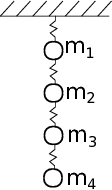
\includegraphics{../lecture_09/mass_springs.png}
\caption{Springs-masses}
\end{figure}

The masses haves the following amounts, 1, 2, 3, and 4 kg for masses
1-4. Using a FBD for each mass:

\(m_{1}g+k_{2}(x_{2}-x_{1})-k_{1}x_{1}=0\)

\(m_{2}g+k_{3}(x_{3}-x_{2})-k_{2}(x_{2}-x_{1})=0\)

\(m_{3}g+k_{4}(x_{4}-x_{3})-k_{3}(x_{3}-x_{2})=0\)

\(m_{4}g-k_{4}(x_{4}-x_{3})=0\)

in matrix form:

\(\left[ \begin{array}{cccc} k_{1}+k_{2} & -k_{2} & 0 & 0 \\ -k_{2} & k_{2}+k_{3} & -k_{3} & 0 \\ 0 & -k_{3} & k_{3}+k_{4} & -k_{4} \\ 0 & 0 & -k_{4} & k_{4} \end{array} \right] \left[ \begin{array}{c} x_{1} \\ x_{2} \\ x_{3} \\ x_{4} \end{array} \right]= \left[ \begin{array}{c} m_{1}g \\ m_{2}g \\ m_{3}g \\ m_{4}g \end{array} \right]\)

    \begin{Verbatim}[commandchars=\\\{\}]
{\color{incolor}In [{\color{incolor}21}]:} \PY{n}{k1}\PY{p}{=}\PY{l+m+mi}{10}\PY{p}{;} \PY{c}{\PYZpc{} N/m}
         \PY{n}{k2}\PY{p}{=}\PY{l+m+mi}{100000}\PY{p}{;}
         \PY{n}{k3}\PY{p}{=}\PY{l+m+mi}{10}\PY{p}{;}
         \PY{n}{k4}\PY{p}{=}\PY{l+m+mi}{1}\PY{p}{;}
         \PY{n}{m1}\PY{p}{=}\PY{l+m+mi}{1}\PY{p}{;} \PY{c}{\PYZpc{} kg}
         \PY{n}{m2}\PY{p}{=}\PY{l+m+mi}{2}\PY{p}{;}
         \PY{n}{m3}\PY{p}{=}\PY{l+m+mi}{3}\PY{p}{;}
         \PY{n}{m4}\PY{p}{=}\PY{l+m+mi}{4}\PY{p}{;}
         \PY{n}{g}\PY{p}{=}\PY{l+m+mf}{9.81}\PY{p}{;} \PY{c}{\PYZpc{} m/s\PYZca{}2}
         \PY{n}{K}\PY{p}{=}\PY{p}{[}\PY{n}{k1}\PY{o}{+}\PY{n}{k2} \PY{o}{\PYZhy{}}\PY{n}{k2} \PY{l+m+mi}{0} \PY{l+m+mi}{0}\PY{p}{;} \PY{o}{\PYZhy{}}\PY{n}{k2} \PY{n}{k2}\PY{o}{+}\PY{n}{k3} \PY{o}{\PYZhy{}}\PY{n}{k3} \PY{l+m+mi}{0}\PY{p}{;} \PY{l+m+mi}{0} \PY{o}{\PYZhy{}}\PY{n}{k3} \PY{n}{k3}\PY{o}{+}\PY{n}{k4} \PY{o}{\PYZhy{}}\PY{n}{k4}\PY{p}{;} \PY{l+m+mi}{0} \PY{l+m+mi}{0} \PY{o}{\PYZhy{}}\PY{n}{k4} \PY{n}{k4}\PY{p}{]}
         \PY{n}{y}\PY{p}{=}\PY{p}{[}\PY{n}{m1}\PY{o}{*}\PY{n}{g}\PY{p}{;}\PY{n}{m2}\PY{o}{*}\PY{n}{g}\PY{p}{;}\PY{n}{m3}\PY{o}{*}\PY{n}{g}\PY{p}{;}\PY{n}{m4}\PY{o}{*}\PY{n}{g}\PY{p}{]}
\end{Verbatim}

    \begin{Verbatim}[commandchars=\\\{\}]
K =

   100010  -100000        0        0
  -100000   100010      -10        0
        0      -10       11       -1
        0        0       -1        1

y =

    9.8100
   19.6200
   29.4300
   39.2400


    \end{Verbatim}

    \begin{Verbatim}[commandchars=\\\{\}]
{\color{incolor}In [{\color{incolor}25}]:} \PY{n+nb}{cond}\PY{p}{(}\PY{n}{K}\PY{p}{,}\PY{n+nb}{inf}\PY{p}{)}
         \PY{n+nb}{cond}\PY{p}{(}\PY{n}{K}\PY{p}{,}\PY{l+m+mi}{1}\PY{p}{)}
         \PY{n+nb}{cond}\PY{p}{(}\PY{n}{K}\PY{p}{,}\PY{l+s}{\PYZsq{}}\PY{l+s}{fro\PYZsq{}}\PY{p}{)}
         \PY{n+nb}{cond}\PY{p}{(}\PY{n}{K}\PY{p}{,}\PY{l+m+mi}{2}\PY{p}{)}
\end{Verbatim}

    \begin{Verbatim}[commandchars=\\\{\}]
ans =    3.2004e+05
ans =    3.2004e+05
ans =    2.5925e+05
ans =    2.5293e+05

    \end{Verbatim}

    \begin{Verbatim}[commandchars=\\\{\}]
{\color{incolor}In [{\color{incolor}26}]:} \PY{n+nb}{e}\PY{p}{=}\PY{n+nb}{eig}\PY{p}{(}\PY{n}{K}\PY{p}{)}
         \PY{n+nb}{max}\PY{p}{(}\PY{n+nb}{e}\PY{p}{)}\PY{o}{/}\PY{n+nb}{min}\PY{p}{(}\PY{n+nb}{e}\PY{p}{)}
\end{Verbatim}

    \begin{Verbatim}[commandchars=\\\{\}]
e =

   7.9078e-01
   3.5881e+00
   1.7621e+01
   2.0001e+05

ans =    2.5293e+05

    \end{Verbatim}

    \begin{Verbatim}[commandchars=\\\{\}]
{\color{incolor}In [{\color{incolor} }]:} 
\end{Verbatim}


    % Add a bibliography block to the postdoc
    
    
    
    \end{document}
